%
% File acl2019.tex
%
%% Based on the style files for ACL 2018, NAACL 2018/19, which were
%% Based on the style files for ACL-2015, with some improvements
%%  taken from the NAACL-2016 style
%% Based on the style files for ACL-2014, which were, in turn,
%% based on ACL-2013, ACL-2012, ACL-2011, ACL-2010, ACL-IJCNLP-2009,
%% EACL-2009, IJCNLP-2008...
%% Based on the style files for EACL 2006 by 
%%e.agirre@ehu.es or Sergi.Balari@uab.es
%% and that of ACL 08 by Joakim Nivre and Noah Smith

\documentclass[11pt,a4paper]{article}
\usepackage[hyperref]{acl2019}
\usepackage{times}
\usepackage{latexsym}
\usepackage{amsmath}
\usepackage{graphicx}
\usepackage{caption}
\usepackage{subcaption}
\usepackage{hyperref}

\usepackage{relsize}
\renewcommand*{\UrlFont}{\smaller\relax}


\DeclareMathOperator*{\argmax}{arg\,max}
\DeclareMathOperator*{\argmin}{arg\,min}
\usepackage{enumitem}


\usepackage{url}

\aclfinalcopy % Uncomment this line for the final submission
%\def\aclpaperid{***} %  Enter the acl Paper ID here

%\setlength\titlebox{5cm}
% You can expand the titlebox if you need extra space
% to show all the authors. Please do not make the titlebox
% smaller than 5cm (the original size); we will check this
% in the camera-ready version and ask you to change it back.
\newcommand\BibTeX{B\textsc{ib}\TeX}

\title{Concept Tagging for the Movie Domain by using Tranfer Learning and Named Entity Recognition.}

\author{Giovanni De Toni (197814) \\
  University of Trento \\ Via Sommarive, 9, 38123 Povo,Trento TN\\
  \texttt{giovanni.detoni@studenti.unitn.it}}

\date{}

\begin{document}
\maketitle

\begin{abstract}
la
\end{abstract}

\section{Introduction}
Concept Tagging sequence is a classical problem in the NLP field. It consists of assigning to each word of a sentence a given concept which represents the meaning of that word (e.g., ``star wars" is a movie title, ``movie.title"). Over the past years, it was extensively studied and several techniques were developed such to efficiently tag words given a pool of concepts. The most basic methods are statistical language models (Weight Finite State Automa) which are easy to train and yield quite impressive results. However, with the rise of neural networks and, in particular, recurrent neural networks, we can train models which have better performances than their statistic counterparts. Moreover, thanks to the use of specific word embeddings (e.g., word2vec, GloVe, etc.), we were able to boost the performances even more.
This work takes as a starting point the paper of Gobbi et. all [add citation] and it tries to improve the scores of some of the neural models presented there, by adding new features and by trying to employ more intelligent embeddings. The report is structured as follow: the first section formalizes the problem statement, the second section describes the corpora used and the third section describes the model tested and evaluated. Ultimately,  the fourth and fifth section reports the experiments performed and the final results.  	

\section{Models}

To evaluate how the performance changes with respect to the previous results we selected four models from the original work. We concentrated on the neural networks approaches by selecting the ones which held the best results over the test set. We chose the following architectures: LSTM, LSTM-CRF, LSTM-CHAR-REP and LSTM-CRF-CHAR-REP. 
Moreover, we extended the features used by the various models by providing also the POS tags and the NER entities as one-hot-encoded vectors. 
To account for possible differences in the environment between our implementation and the original work we also tried to replicate the original results for those architectures. We then checked the results against the baseline provided in the original paper.

Long-Short Term Memor (LSTM) [add citation] is a model which extends and improve the previous RNN by solving the vanishing/exploding gradients. We tested a simple LSTM which receives in input the embeddings of the words (plus other features like the POS tags and the NER tags). Moreover, we tested another LSTM model which uses also the characters embeddings obtained using a convolutional layer (LSTM-CHAR-REP). 
We experimented also with the LSTM-CRF model [add citation] in which the LSTM provides the class scores for each token and then the Viterbi algorithm is used to determine the labels at a global level. This model was also tested by adding more features (POS and NER tags). Moreover, an LSTM-CRF version extended with the characters convolution was also evaluated (LSTM-CRF-CHAR-REP).


\begin{figure*}
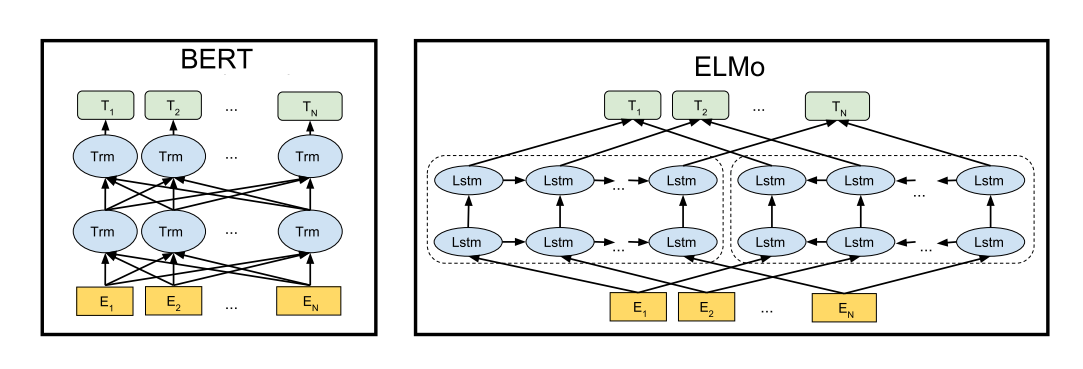
\includegraphics[width=\linewidth]{img/bert-elmo-2.png}
\caption{Graphic representation of the ELMo and BERT architectures. The yellow boxes indicates the tokens sent through the architecture while the green box on the top indicates the resulting embeddings. It can be clearly seen how the ELMo architecture uses instead two LSTMs to analyze the left and right context [add image citation].}
\end{figure*}



\section{Embeddings}

As a first step to improve the performances of the previous work we concentrate on evaluating several recently proposed pre-trained language models to produce words representations or embeddings. Language representations can be either context-free or contextual. 
Context-free means that the word representation is generated without looking at the context in which the word is used. For instance, the word "season" may have different meanings with respect to the context in which it is placed (e.g., "Summer is my favourite season" and "Add some season to the chicken and then serve"), but in a context-free model it will get the same representation (embedding). A contextual representation takes care also of the context in which a word is used.
Moreover, the contextual representations can be further divided into two other categories: unidirectional or bidirectional. 
A unidirectional model contextualizes a given term by just looking at the words on the right (or on the left) of it.  A bidirectional model instead looks both on the left and on the right of the target word before producing a representation. There are also swallow bidirectional models which combines two unidirectional models (one for the left side and one for the right side) to give a more complete representation. In our work, we tested three different embeddings, one for each category (context-free, contextual swallow bidirectional and contextual bidirectional): ConceptNet, ELMo and BERT.

\begin{figure*}[!ht]
\begin{subfigure}{0.5\linewidth}
  \centering
  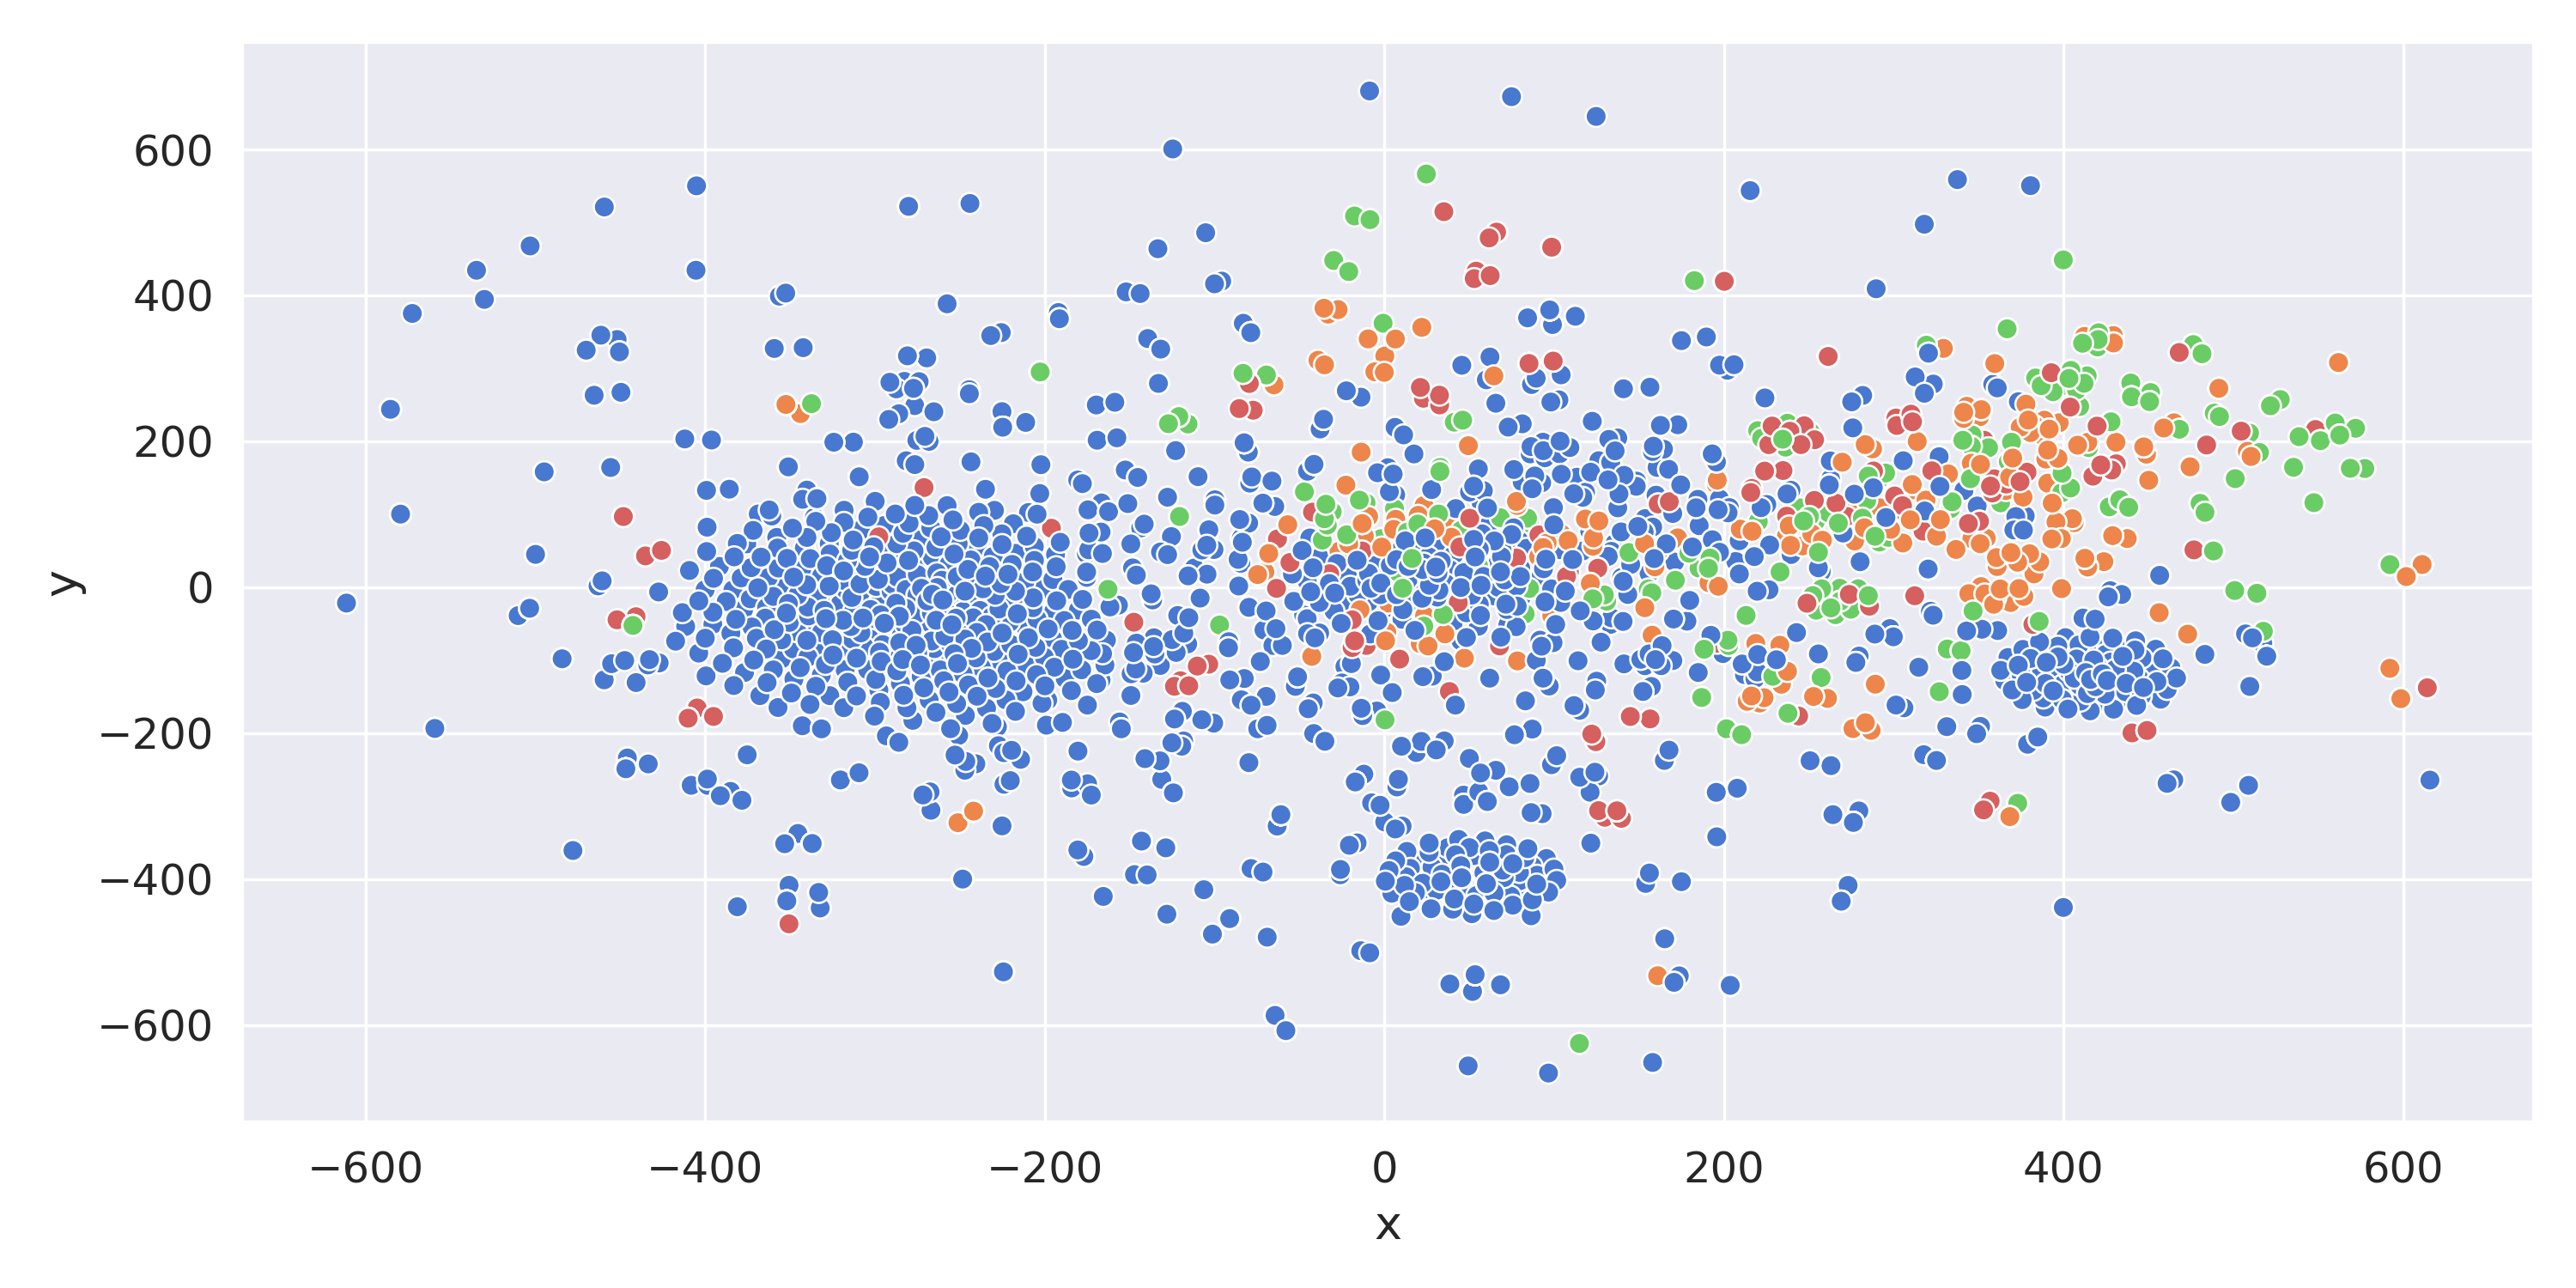
\includegraphics[width=\linewidth]{img/word2vec-embeddings.png}
  \caption{Default Embeddings}
  \label{fig:sfig1}
\end{subfigure}%
\begin{subfigure}{0.5\linewidth}
  \centering
  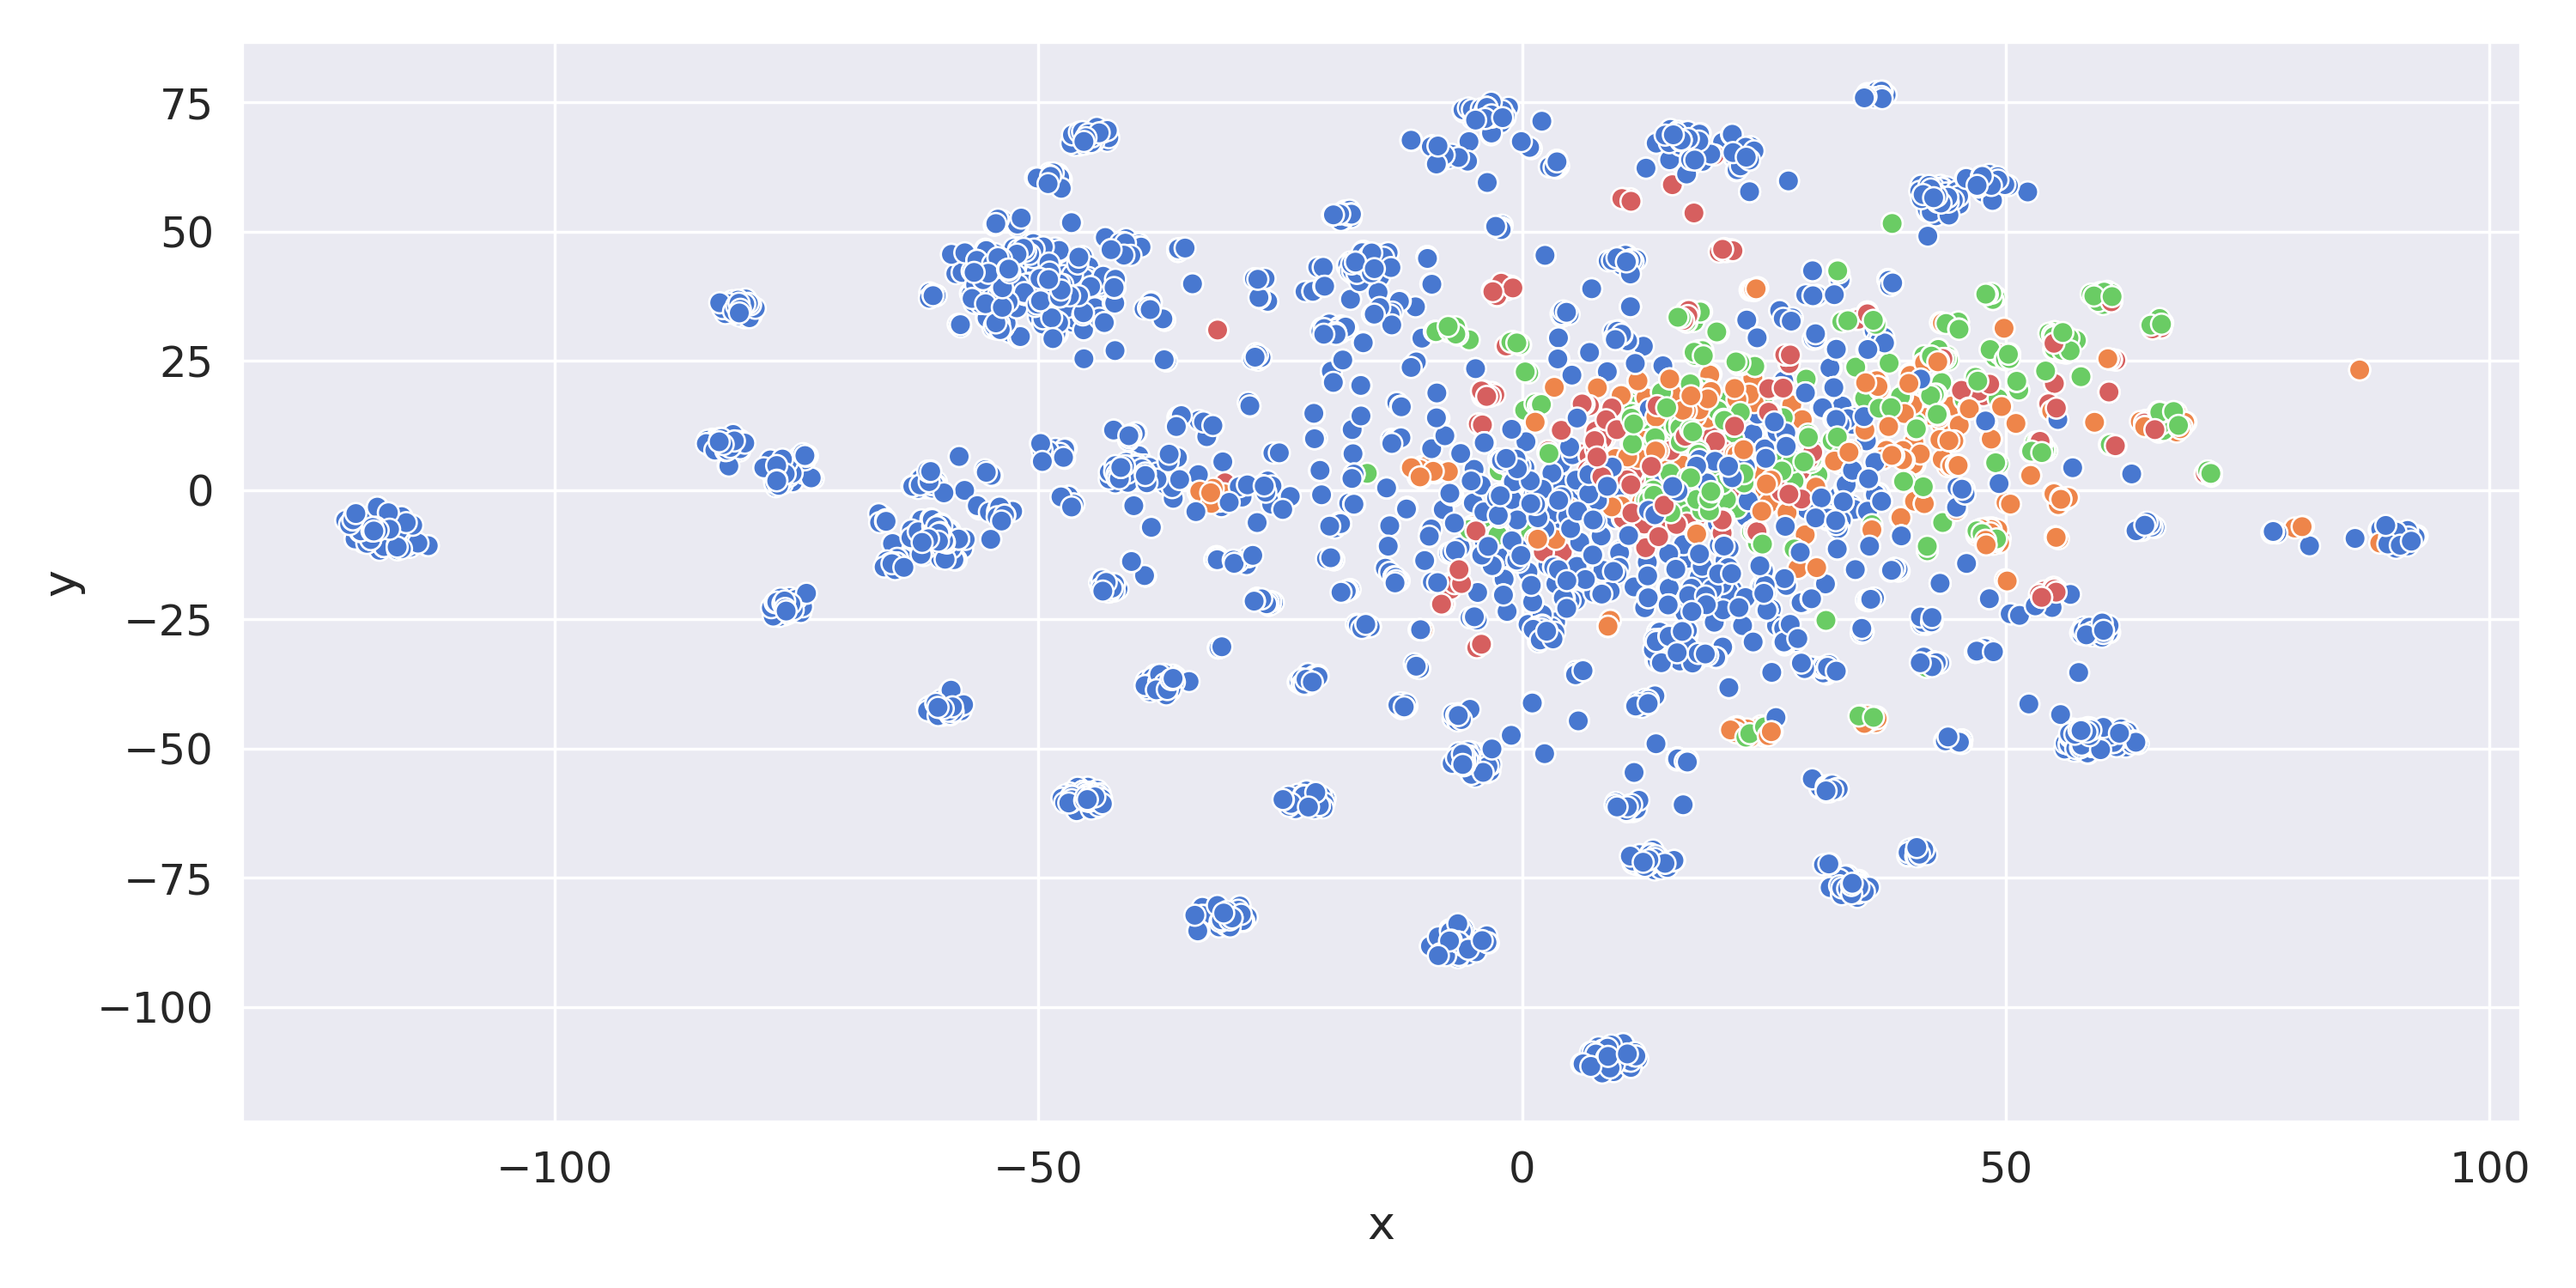
\includegraphics[width=\linewidth]{img/elmo-embeddings.png}
  \caption{Elmo Embeddings}
  \label{fig:sfig2}
\end{subfigure}\\
\begin{subfigure}{0.5\linewidth}
  \centering
  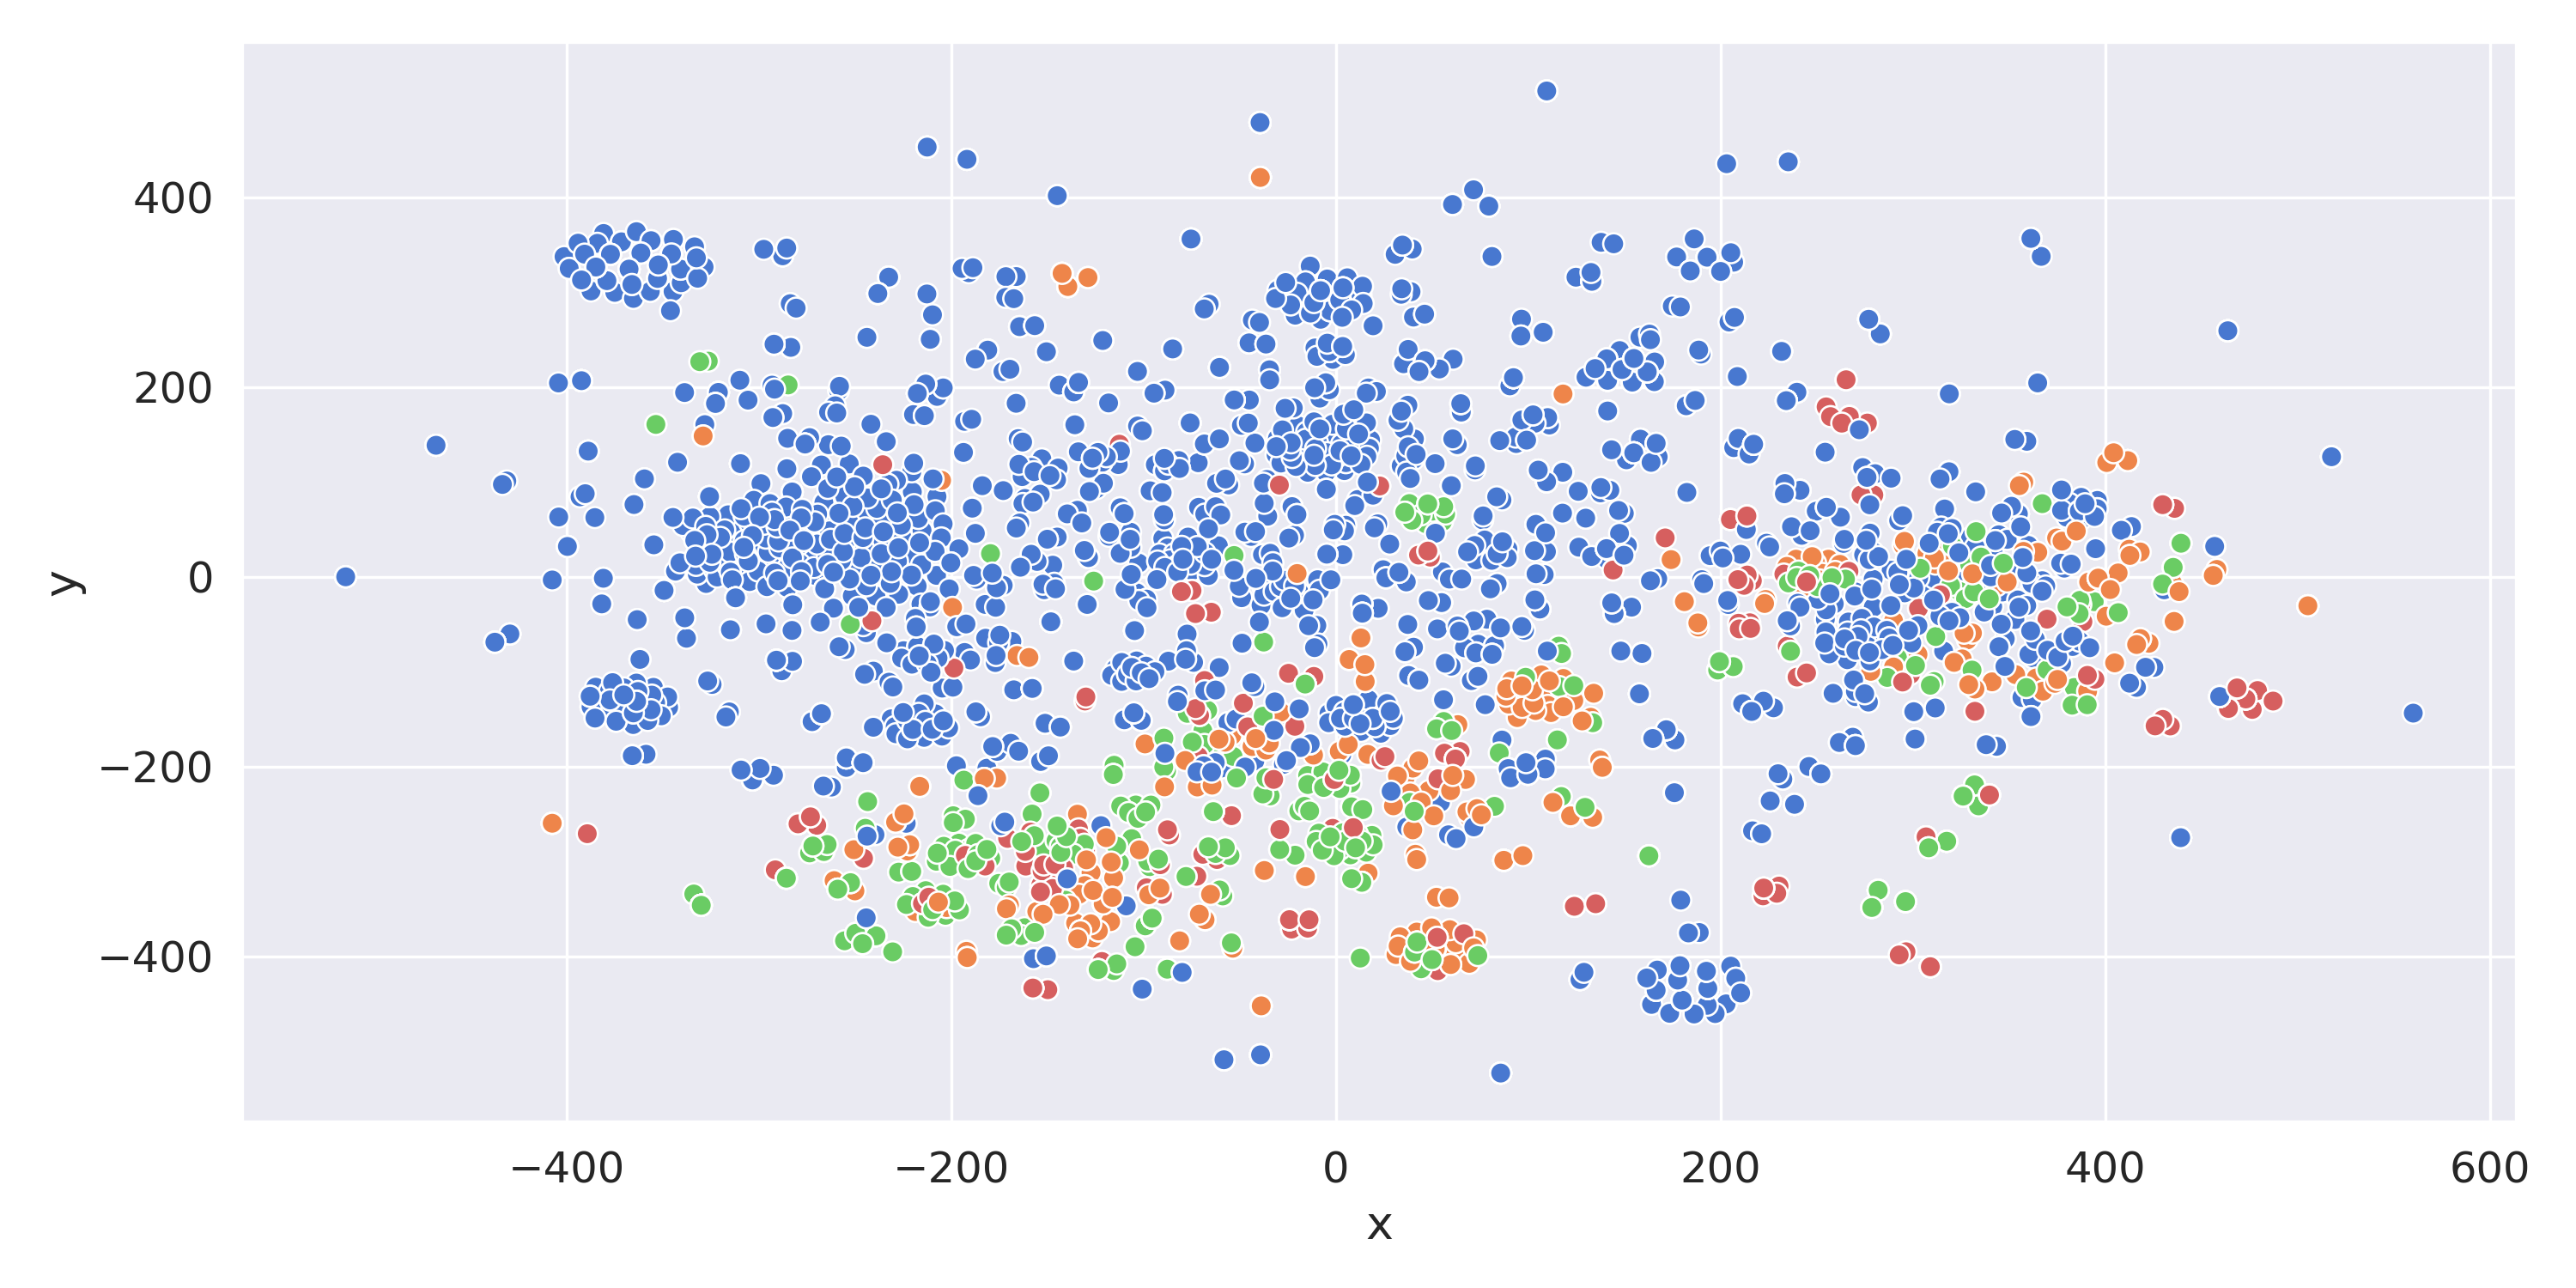
\includegraphics[width=\linewidth]{img/bert-embeddings.png}
  \caption{Bert Embeddings}
  \label{fig:sfig2}
\end{subfigure}%
\begin{subfigure}{0.5\linewidth}
  \centering
  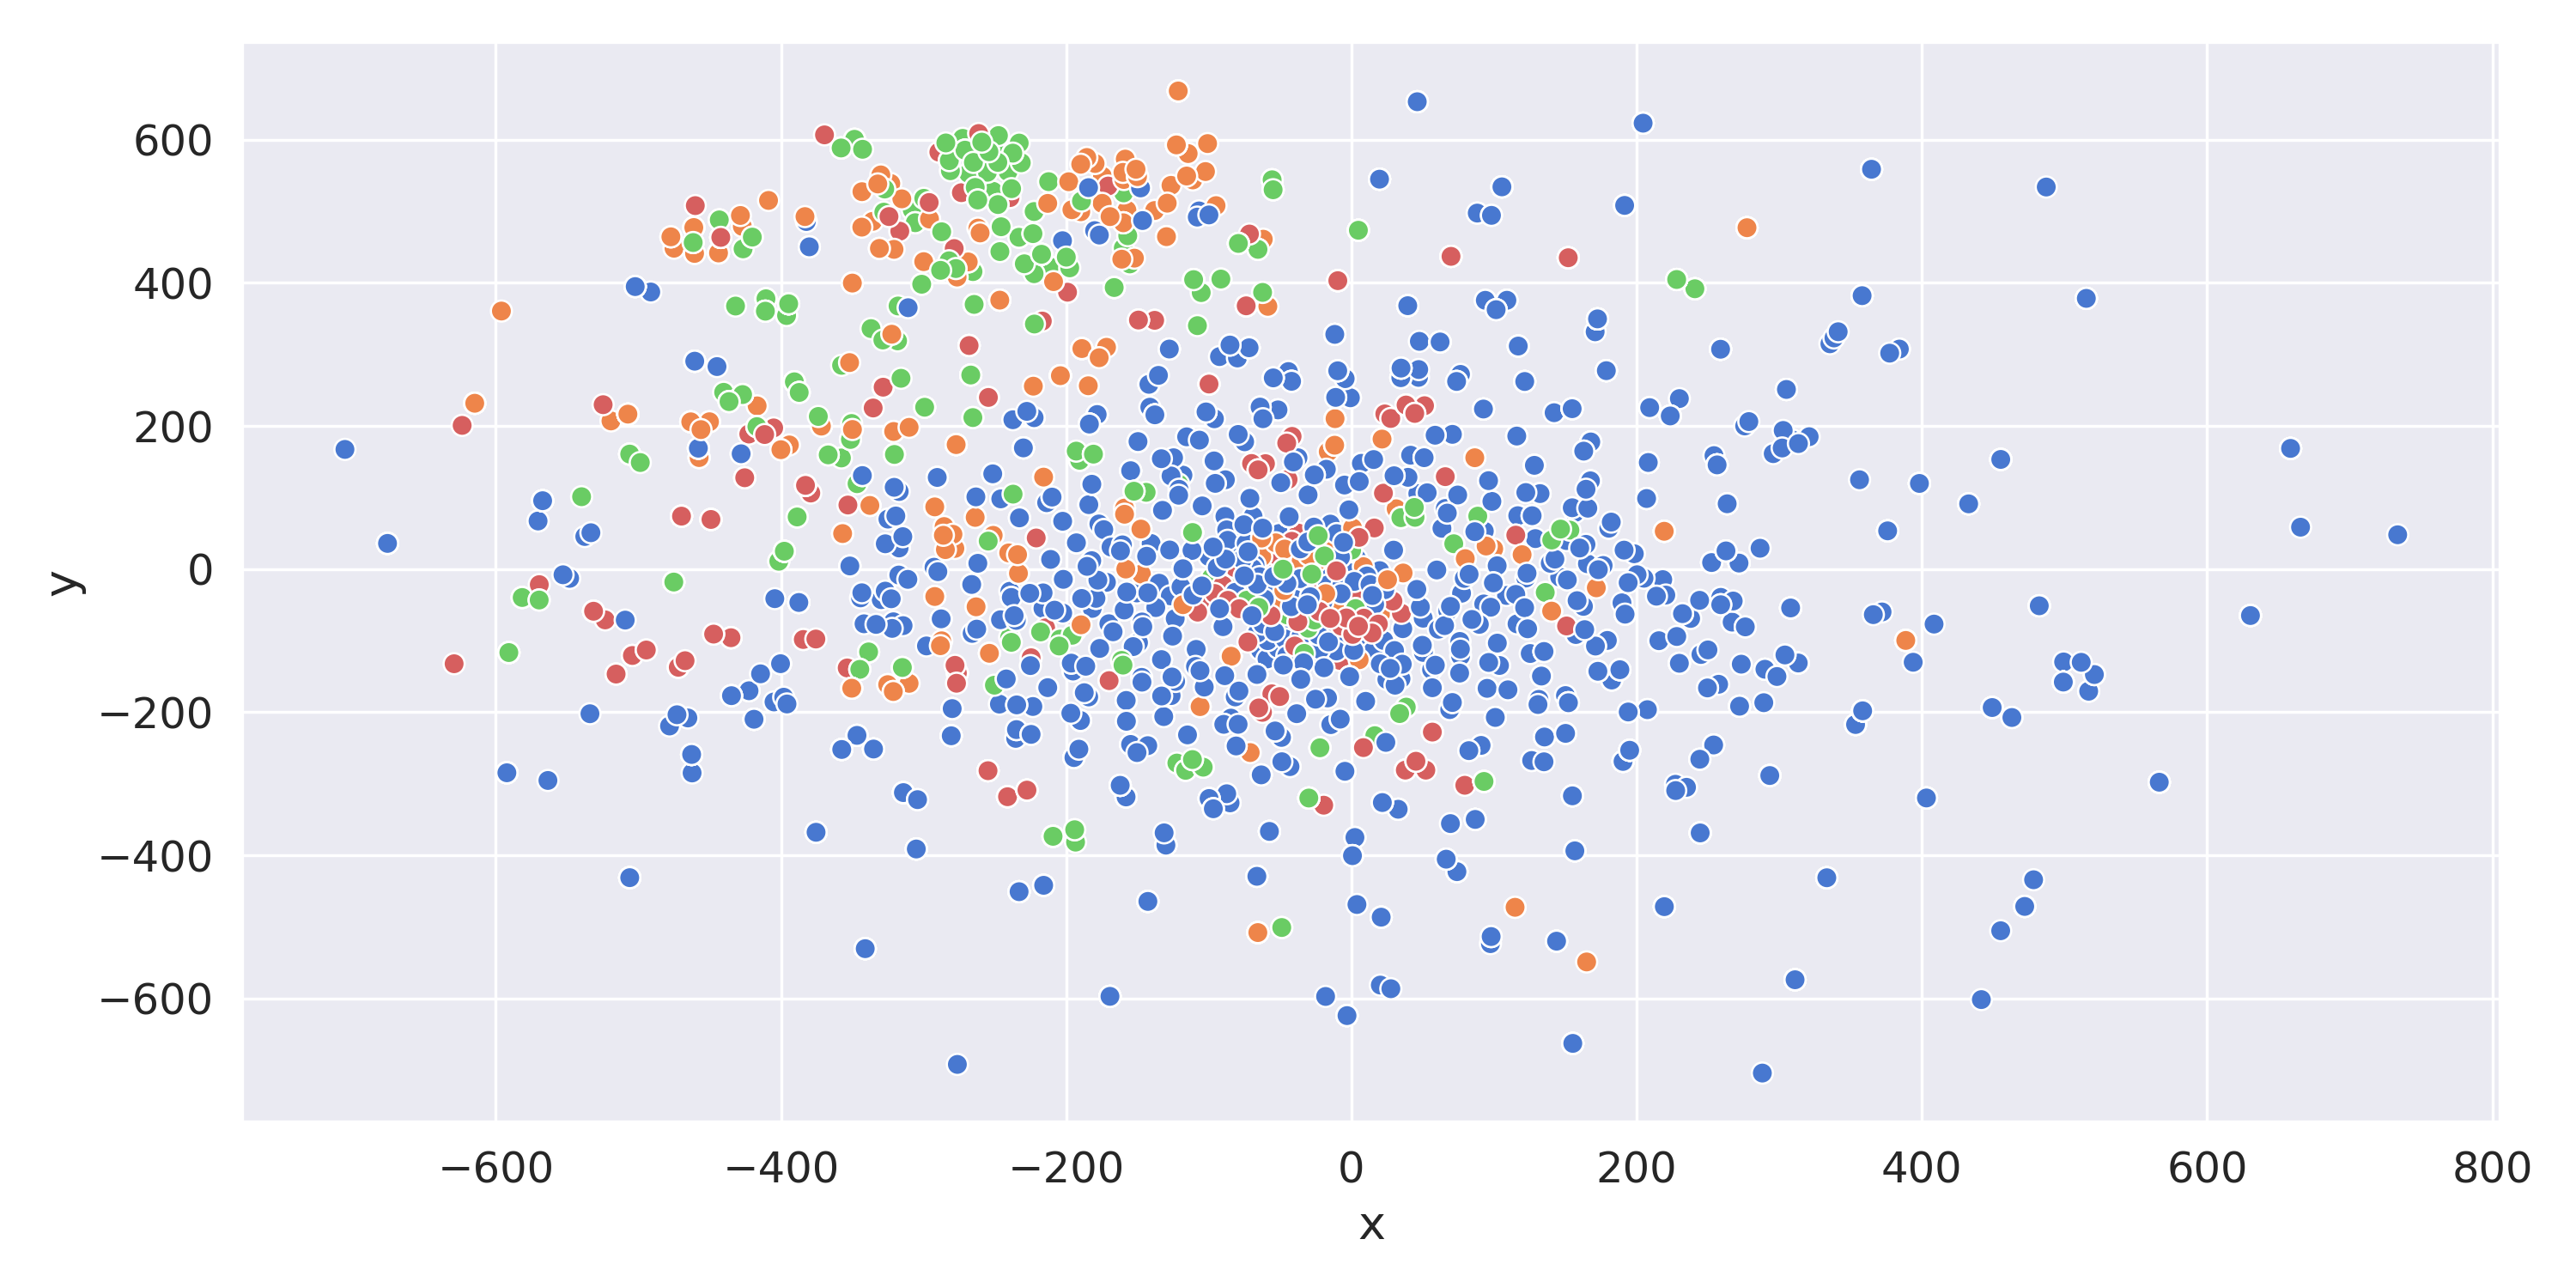
\includegraphics[width=\linewidth]{img/conceptnet-embeddings.png}
  \caption{ConceptNet Embeddings}
  \label{fig:sfig2}
\end{subfigure}
\caption{These plots shows the embeddings representation of the four major concepts of the train dataset. Namely, movie.name (blue), actor.name (orange), producer.name (red) and director.name (green). We can clearly see how some embeddings enable much nicer clusters for some concepts, while others seems not to be able to do it.}
\label{fig:fig}
\end{figure*}

\subsection{ConceptNet}
ConceptNet Numberbatch [add citation] is a context-free language model. It is a set of word embeddings and it was made by combining previously existing models, namely, GloVe [add citation], word2vec [add citation] and OpenSubtitles 2016 [add citation]. Moreover, it leverages the data of the ConceptNet knowledge graph to enrich its representation. The authors reached this goal by using a retrofitting procedure [add citation faruqui] to adjust the word embedding matrix by using their knowledge graph. Thanks to this procedure, ConceptNet is also intrinsically multilingual since this method pushes the model to use the same embedding space both for English words and words in different languages (since they share the same meaning).  This work uses the Numberbatch 19.08 English-only model which contains 516782 embeddings of size 300. 


\subsection{ELMo}
ELMo [add citation] is a deep contextualized word representation which captures both syntactic, semantic and polysemy characteristics of a given word. It uses a deep shallow bidirectional language model (biLM) trained on a large corpus. The ELMo method differs from the classical context-free approaches (e.g., GloVe, word2vec, fastText, etc.) because each word embedding is obtained by looking at the entire input sentence.  The generated representation are deep because they are a function of all the layers of the biLM. Moreover, each layer models certain features of the given word. The original work states that the higher-level LSTM states capture context-dependent aspects of the word meaning, while lower-level states capture aspects of the syntax.
We used the pre-trained small ELMo model [add citation] with the dimension of the embedding of 1024.
In this work, we run ELMo and we recorded all the layer representation of each word of each sentence in the training dataset. We then devised two strategies to combine them to obtain the final embeddings. The first strategy produces a linear combination given an equal weighting over the three layers. In the second strategy, the weights of the linear combination are directly learned with all the other parameters. 


\subsection{BERT}

BERT (Bidirectional Encoder Representations from Transformers) [add citation] is a relatively new language representation model released in 2019. It pre-trains deep bidirectional representations from unlabeled texts by exploiting both the left and right context. The model is a multi-layer bidirectional Transformer encoder. The authors state that this new representation solves the previous limitations of pre-trained models (e.g., ELMo). They argue that the standard LMs are unidirectional, thus limiting the kind of architectures which can be used during training. Moreover, such architectures could produce sub-optimal performances on tasks where it is important to fuse context from both directions. 
There are two steps in the BERT framework: pre-training and fine-tuning. During the first phase, the model is trained on unlabeled data over two separate unsupervised training tasks: Masked LM and Next Sentence Prediction (NSP).  The Masked LM task consists of predicting some works of the given input phrase which are masked beforehand.  This would enable to train a real deep bidirectional representation since bidirectional conditioning on standard LM is not possible. The Next Sentence Prediction (NSP) consists of prediction relationships between sentences which are usually not captured by LM. 
During the fine-tuning phase, the model is initialized with the pre-trained parameters obtained in the previous stage and it is fine-tuned on the desired task. 

In our work, we used a pre-trained BERT model to get the word embeddings directly without doing the pre-training phase [https://pypi.org/project/bert-embedding/]. More specifically, the BERT model used was pre-trained on the BookCorpus [add citation] and English Wikipedia. The embedding dimension was 768. 



\section{Data Analysis}

Following the original implementation, we evaluated our solutions by using the NL2SparQL4NLU dataset [add citation]. It corresponds to the MOVIE dataset of the original paper. It includes mainly sentences taken from the movie domain (e.g.,``trailer for star wars a new hope"). The dataset contains 3338 and 1084 sentences for the train and test set respectively. The dictionary size (\# of unique tokens) is of 1728 and 1039  (again training and test set). The average sentence length is 6.42 and 6.52 with an OOV rate between the datasets of 24\%. We have a total of 23 concepts over the entire (with a total of 43 concepts in IOB format). Each word was POS tagged and there are 50 different tags between the training and test set (taken from the Tree Tagger POS list [add citation]). Moreover, each sentence was also analyzed using a Named Entity Recognition (NER) tool, spaCy [add citation], which found 9 different entities in 398 (1,86\%)  and 169 (2,37\%) tokens for the training and test set respectively.

\section{Embedding Analysis}
We evaluated also the various embeddings presented before. For the ConceptNet we analyzed the embedding coverage (namely, how many words in the dataset dictionary can be found in the embedding matrix) and we compared it with the embedding used in the baseline. For BERT and ELMo models we did a visual analysis instead. More specifically, we used T-sne (add citation) to reduce the dimensionality of the BER/ELMo embeddings down to 2D and then we plotted the results for the four most represented concepts in the dataset. We did the same for the classical ConceptNet and default embeddings.

\textbf{Description of the dataset}

\textbf{Description of spacy and pos as features}

\textbf{Comparison of the embeddings}

\section{Experiments}



\section{Results}

%\bibliography{acl2019}
%\bibliographystyle{acl_natbib}

\end{document}
